\documentclass[12pt]{beamer}

\usetheme{CambridgeUS}
\usecolortheme{beaver}
\setbeamertemplate{navigation symbols}{}

\usepackage[utf8]{inputenc}
\usepackage{listings}
\usepackage{caption}

\usepackage{tikz}
\usetikzlibrary{trees}

%\usepackage[croatian]{babel}
\usepackage{hyperref}

\date{}


\title[]{RasPitaj se!\\Radni okvir Flask}
\author[Leonard Volarić Horvat, ICM]{Leonard Volarić Horvat, ICM}

\institute[FER]{Sveučilište u Zagrebu\\Fakultet elektrotehnike i računarstva}

\begin{document}

{
	%\setbeamertemplate{headline}[]
	%\setbeamertemplate{footline}{}
	\begin{frame}
		\maketitle
	\end{frame}
}

\begin{frame}
	Sadržaj:
	\tableofcontents
\end{frame}

\section{Python}
\begin{frame}
\frametitle{Python}
	\begin{itemize}
		\item Vrlo popularan programski jezik
		\item Odlike:
		\begin{itemize}
			\item Jednostavna sintaksa (pravila pisanja)
			\item Proširivost
			\item Vrlo raširena i pristupačna zajednica korisnika
		\end{itemize}
		\item Trenutno dostupne verzije: Python2 i Python3
	\end{itemize}
\end{frame}

\subsection{Proširivost}
\begin{frame}
	\frametitle{Proširivost - biblioteke}
	\begin{itemize}
		\item Na internetu dostupno puno biblioteka opće i specifične namjene
		\item Primjeri: numpy, reportpdf, \textbf{flask}
		\item Instalacija: \textbf{pip}
	\end{itemize}
\end{frame}

\subsection{pip}
\begin{frame}
	\frametitle{pip}
	\begin{itemize}
		\item \textit{Package manager} za Python
		\item Program za instalaciju paketa/biblioteka
		\item python 2: pip; python3: pip3
		\item Instalacija: \textit{sudo apt install pip(3)}
		\item Korištenje: pip(3) install flask
	\end{itemize}
\end{frame}

\section{Virtualne okoline}
\begin{frame}
	\frametitle{Virtualne okoline}
	\begin{itemize}
		\item Veći projekti koriste više paketa
		\item U međuvremenu se paketi ažuriraju
		\item Nekada ažuriranja "strgaju stvari"
		\item Projekti možda iziskuju međusobno različite inačice paketa
		\item \rigtharrow trebamo način za "higijensko" upravljanje paketima
	\end{itemize}

	Koristit ćemo \href{http://virtualenvwrapper.readthedocs.io/}{\textit{virtualenvwrapper}}
\end{frame}

\section{Flask}
\begin{frame}
	\frametitle{Flask}
	\begin{itemize}
		\item Jednostavan radni okvir (\textit{framework}) za razvoj web aplikacija
		\item Uređena i lako pratljiva hijerarhija datoteka
		\item Lagan i brz razvoj
	\end{itemize}
\end{frame}

\subsection{Struktura flask projekta}
\begin{frame}
	\frametitle{Struktura projekta}
	\tikzstyle{every node}=[draw=black,thick,anchor=west]
	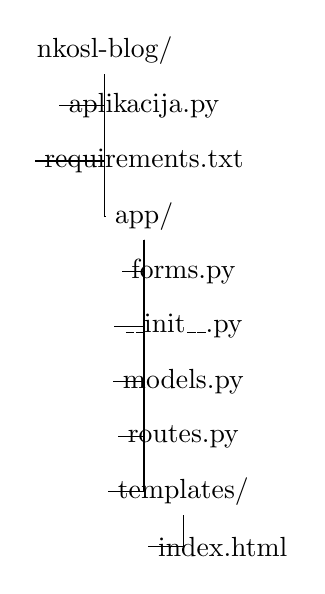
\begin{tikzpicture}[%
		grow via three points={one child at (0.5,-0.7) and
		two children at (0.5,-0.7) and (0.5,-1.4)},
		edge from parent path={(\tikzparentnode.south) |- (\tikzchildnode.west)}]
		\node {nkosl-blog/}
			child { node {aplikacija.py}}
			child { node {requirements.txt}}
			child { node {app/}
				child { node {forms.py}}
				child { node {\_\_init\_\_.py}}
				child { node {models.py}}
				child { node {routes.py}}
				child { node {templates/}
					child { node {index.html}}
				}
			};
	\end{tikzpicture}\\
\end{frame}


% \begin{frame}
% 	\begin{itemize}
% 		\item
% 	\end{itemize}
% \end{frame}
\end{document}